\documentclass[11pt,a4paper]{article}

% Packages
\usepackage[utf8]{inputenc}
\usepackage{graphicx}
\usepackage{booktabs}
\usepackage{amsmath}
\usepackage{siunitx}
\usepackage{hyperref}
\usepackage{xcolor}
\usepackage{geometry}
\usepackage{listings}
\usepackage{caption}
\usepackage[section]{placeins}
\usepackage{float}
\geometry{margin=1in}

% Configure listings for XML
\lstdefinestyle{xmlstyle}{
    language=XML,
    backgroundcolor=\color{gray!10},
    basicstyle=\small\ttfamily,
    breaklines=true,
    frame=single,
    showspaces=false,
    showstringspaces=false,
    keywordstyle=\color{blue},
    commentstyle=\color{green!60!black},
    stringstyle=\color{red},
    morekeywords={mujoco,worldbody,light,body,joint,geom,name,pos,euler,type,axis,size,rgba}
}

\title{A Comparison of GPU vs CPU Based Physics Engines}
\author{Rory Edmonds}
\date{\today}

\begin{document}

\maketitle

%\begin{abstract}

%\end{abstract}

\section{Introduction}
This report presents a benchmarking study of several modern physics engines for simulating articulated robots. We evaluate Mujoco, MJX, Genesis, and Newton (with XPBD, Featherstone, and MJWarp solvers) across various batch sizes and test cases. The aim of this is to provide insights into their performance across a range of simulation tasks to aid in selecting the most suitable engine for the task at hand. The parallelisation provided by GPU-based physics engines lends itself to high throughput simulation tasks, such as reinforcement learning and trajectory optimisation, where many environments need to be simulated simultaneously. In this report, we focus on the performance of these engines in terms of speed, particularly when scaling to large batch sizes, but we will not discount the importance of physical accuracy when looking at the results.

\section{Physics Engines Overview}
\subsection{Mujoco}
Mujoco is the only CPU-based engine we will be evaluating. This is because it is the industry standard for simulating articulated robots, and it is widely used in reinforcement learning research. It uses a continuous-time formulation of dynamics, which allows for high accuracy in simulation. 
\subsection{MJX}
MJX is a GPU-accelerated variant of MuJoCo developed by Google DeepMind. It is designed to work seamlessly with JAX, allowing for efficient automatic differentiation and parallel execution on GPUs. MJX retains the core features of MuJoCo while providing significant performance improvements for large-scale simulations.
\subsection{Genesis}
Genesis is a high-performance GPU physics engine designed to be lightweight, usable and capable of simulating a wide-range of materials and phenomena. It provides a unified framework for several different solvers, although we will just be focusing on rigid body dynamics in this report. 

\subsection{Newton}
Newton is a physics engine that supports multiple solvers, including XPBD, Featherstone, and MJWarp. It is designed to be flexible and efficient, allowing for high-performance simulations on both CPU and GPU. It leverages NVIDIA's warp technology to accelerate physics computations, making it suitable for large-scale simulations.
\subsubsection{XPBD Solver}
The XPBD solver is a position-based dynamics solver, this means it doesn't solve the full dynamics equations, but instead iteratively adjusts positions to satisfy constraints. This allows for fast and stable simulations, however, it may not be as accurate as other solvers. It is particularly well-suited for simulations where speed is more critical than accuracy, such as in reinforcement learning tasks.
\subsubsection{Featherstone Solver}
The Featherstone solver is an articulated body algorithm that provides efficient and accurate dynamics for multi-body systems. It has high-fidelity and doesn't use a sparse matrix approach.
\subsubsection{MJWarp}
MJWarp is a warp-based solver inspired by MuJoCo, designed to take advantage of GPU parallelism. It uses a similar approach to MuJoCo but is optimised for GPU execution, allowing for high throughput simulations, it is currently under active development and as a result has had several issues whilst testing, but it shows promise for future applications.

\subsection{Hardware}
\begin{itemize}
    \item OS: Ubuntu 24.04
    \item GPU: NVIDIA GeForce RTX 3090 
    \item CPU: Intel i9-11900 @ 2.50GHz
    \item RAM: 125.6 GiB
    \item CUDA: 12.2
\end{itemize}

\subsection{Metrics}
\begin{itemize}
    \item Time to complete simulation (seconds)
    \item FPS per environment
    \item Total FPS across all environments
\end{itemize}

\section{Tests}
\subsection{Simple Pendulum Test}
We use a simple pendulum model to test a simple case of articulation. The pendulum consists of a mass attached to a rigid rod and acts under gravity. We tested several total timestep values with these being split amongst all the environments.

\begin{lstlisting}[style=xmlstyle, caption={Pendulum XML model}, label=lst:pendulum_xml]
<mujoco>
<worldbody>
    <light name="top" pos="0 0 1"/>
    <body name="box_and_sphere" euler="0 0 -30">
    <joint name="swing" type="hinge" axis="1 -1 0" pos="-.2 -.2 -.2"/>
    <geom name="red_box" type="box" size=".2 .2 .2" rgba="1 0 0 1"/>
    <geom name="green_sphere" pos=".2 .2 .2" size=".1" rgba="0 1 0 1"/>
    </body>
</worldbody>
</mujoco>
\end{lstlisting}

\subsubsection{Test Parameters}
\begin{itemize}
    \item \textbf{Time step:} 0.01s
    \item \textbf{Batch sizes:} 
    \begin{itemize}
        \item CPU: 8 cores 
        \item GPU: 2048, 4096, 8192
    \end{itemize}
    \item \textbf{Number of simulation steps:} varied logarithmically between $10^5$ and $10^9$
\end{itemize}

\subsection{Increasing Clutter Test}
In this test we increased the amount of objects in the scene from 1,5,10 and 20. The objects do not collide with anything and just fall under gravity. It is run for a fixed number of steps

\begin{lstlisting}[style=xmlstyle, caption={Pendulum XML model}, label=lst:pendulum_xml]
<mujoco model="random_spheres">
  <option timestep="0.01" gravity="0 0 -9.81" />
  <worldbody>
    <geom name="floor" type="plane" size="50 50 0.1" pos="0 0 0" rgba="0.8 0.8 0.8 1" />
    <body name="sphere_0" pos="1.656 -0.852 0.1">
      <geom type="sphere" size="0.1" rgba="0.2 0.4 0.6 1" />
      <freejoint />
    </body>
    <body name="sphere_1" pos="-1.700 -0.898 0.1">
      <geom type="sphere" size="0.1" rgba="0.2 0.4 0.6 1" />
      <freejoint />
    </body>
    <body name="sphere_2" pos="-1.035 1.277 0.1">
      <geom type="sphere" size="0.1" rgba="0.2 0.4 0.6 1" />
      <freejoint />
    </body>
    <body name="sphere_3" pos="1.372 0.660 0.1">
      <geom type="sphere" size="0.1" rgba="0.2 0.4 0.6 1" />
      <freejoint />
    </body>
    <body name="sphere_4" pos="0.422 1.010 0.1">
      <geom type="sphere" size="0.1" rgba="0.2 0.4 0.6 1" />
      <freejoint />
    </body>
  </worldbody>
</mujoco>
\end{lstlisting}

\subsection{Increasing Contacts Test}
In this test we increased the number of overlapping spheres to see how each solver handles the increasing amount of contacts to resolve. Upon reflection this test is not quite as useful as it could be as once the contact is resolved the spheres do not collide again. Changing this to continually move the spheres into contact would be a better test.

\begin{lstlisting}[style=xmlstyle, caption={Pendulum XML model}, label=lst:pendulum_xml]
<mujoco model="five_contacts">
    <option gravity="0 0 -9.81" integrator="Euler" timestep="0.01"/>
    <size njmax="50" nconmax="50"/>

    <worldbody>
        <!-- Static floor -->
        <geom name="floor" type="plane" pos="0 0 0" size="50 50 0.1" rgba="0.2 0.2 0.2 1" condim="3"/>

        <!-- Cluster of 5 overlapping spheres -->
        <body name="sphere_0" pos="0 0 0.09">
            <geom type="sphere" size="0.1" rgba="1 0 0 1"/>
            <freejoint/>
        </body>

        <body name="sphere_1" pos="0.18 0 0.09">
            <geom type="sphere" size="0.1" rgba="0 1 0 1"/>
            <freejoint/>
        </body>

        <body name="sphere_2" pos="0.09 0.15 0.09">
            <geom type="sphere" size="0.1" rgba="0 0 1 1"/>
            <freejoint/>
        </body>

        <body name="sphere_3" pos="-0.18 0 0.09">
            <geom type="sphere" size="0.1" rgba="1 1 0 1"/>
            <freejoint/>
        </body>

        <body name="sphere_4" pos="0 -0.18 0.09">
            <geom type="sphere" size="0.1" rgba="1 0 1 1"/>
            <freejoint/>
        </body>
    </worldbody>
</mujoco>
\end{lstlisting}

\subsubsection{Test Parameters}
\begin{itemize}
    \item \textbf{Time step:} 0.01s
    \item \textbf{Batch sizes:} 
    \begin{itemize}
        \item CPU: 8 cores 
        \item GPU: 2048, 4096, 8192
    \end{itemize}
    \item \textbf{Number of simulation steps:} $10^6$
    \item \textbf{Number of objects in contacts:} 1, 5, 7, 1s0
\end{itemize}

\subsubsection{Test Parameters}
\begin{itemize}
    \item \textbf{Time step:} 0.01s
    \item \textbf{Batch sizes:} 
    \begin{itemize}
        \item CPU: 8 cores 
        \item GPU: 2048, 4096, 8192
    \end{itemize}
    \item \textbf{Number of simulation steps:} $10^6$
    \item \textbf{Number of objects:} 1, 5, 10, 20
\end{itemize}

\subsection{Articulation Test}
In this test we experimented with how the engines handed a more complex model (The Franka Emika Panda) being manipulated by noisified control signals to mimic machine learning. We tested several total timesteps with these being split amongst all the environments. \\
We used the Franka Emika Panda model from the MJCF repository, which is a common benchmark for articulated robots.

\subsubsection{Test Parameters}
\begin{itemize}
    \item \textbf{Time step:} 0.01s
    \item \textbf{Batch sizes:} 
    \begin{itemize}
        \item CPU: 8 cores 
        \item GPU: 2048, 4096, 8192
    \end{itemize}
    \item \textbf{Number of simulation steps:} varied logarithmically between $10^5$ and $10^9$
\end{itemize}

\subsection{Walker Test}
In this test we experimented with how the engines handed a branching complex model (A simple walker), like with the articulation test, we used noisified control signals to mimic machine learning. We tested several total timesteps with these being split amongst all the environments. \\
We used the Walker model from the MJCF repository, which is a common benchmark for locomotion tasks.

\subsubsection{Test Parameters}
\begin{itemize}
    \item \textbf{Time step:} 0.004s
    \item \textbf{Batch sizes:} 
    \begin{itemize}
        \item CPU: 8 cores 
        \item GPU: 2048, 4096, 8192
    \end{itemize}
    \item \textbf{Number of simulation steps:} varied logarithmically between $10^5$ and $10^9$
\end{itemize}

\section{Results}
\subsection{Simple Pendulum Test}
\FloatBarrier
\begin{figure}[h!]
    \centering
    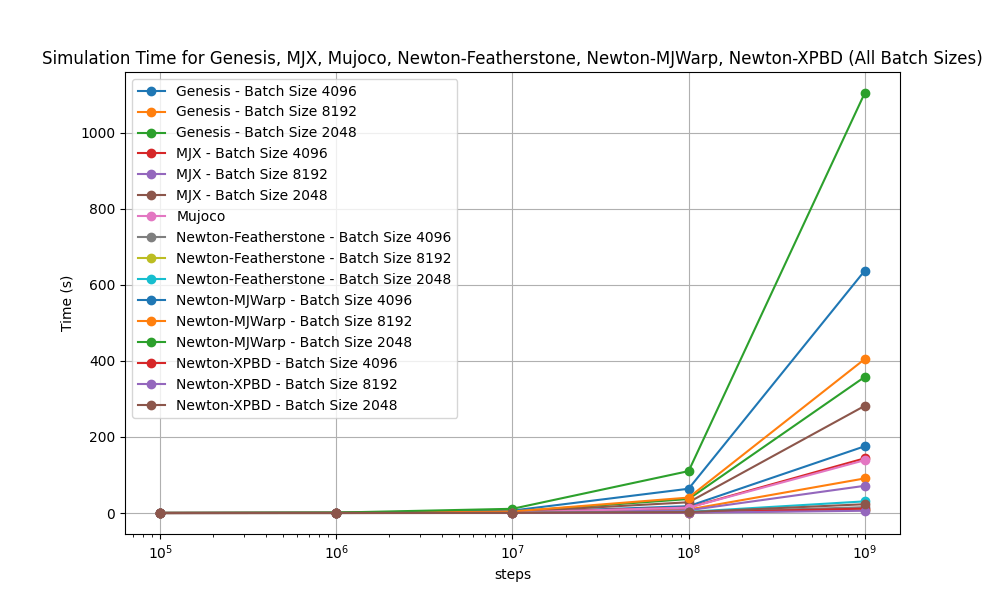
\includegraphics[width=\textwidth]{home/figures/pendulum_speed_all.png}
    \caption{Pendulum Test: Simulation speed comparison across physics engines.}
    \label{fig:pendulum_speed_comparison}
\end{figure}

\FloatBarrier

\subsubsection{Comments:}
Newton's MJWarp did by far the worst out of all the tests.
\begin{figure}[H]
    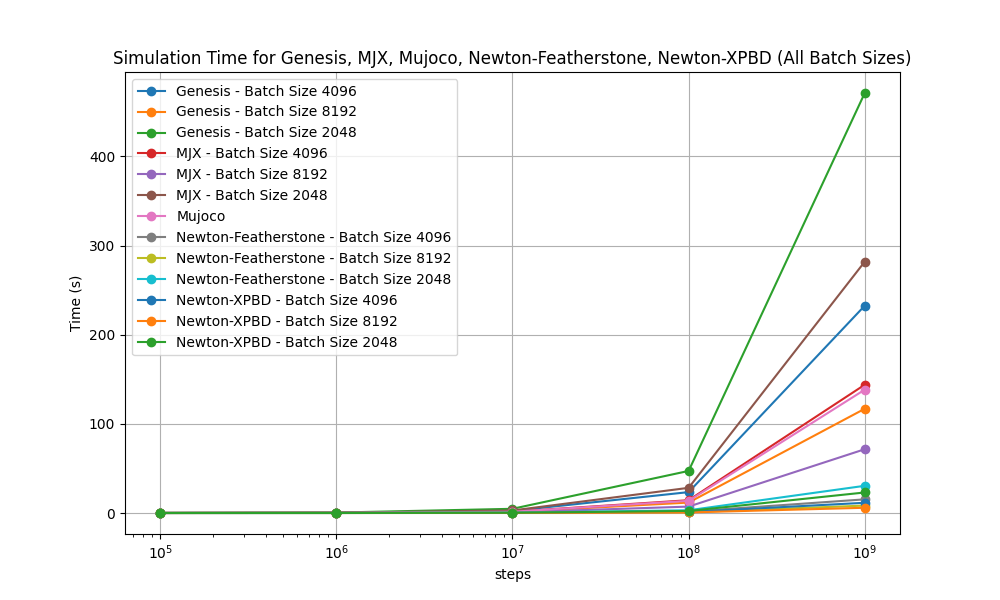
\includegraphics[width=\textwidth]{home/figures/pendulum_speed_no-MJWarp.png}
        \caption{Speed Comparison excluding MJWarp}
    \label{fig:pendulum_speed_comparison_no_MJWarp}
\end{figure}\noindent 
Taking a closer look at the remaining results, we see that Genesis and MJX were of comparable performance, with MJX being much faster at smaller batch sizes but the difference diminishing as batch sizes increase. We also see that MuJoCo is outperformed by both of them (batch size 8192) at the largest step sizes. \\
Featherstone and XPBD for Newton both performed very well, with XPBD being the overall fastest solver.

\subsection{Increasing Clutter Test}
\begin{figure}[H]
    \centering
    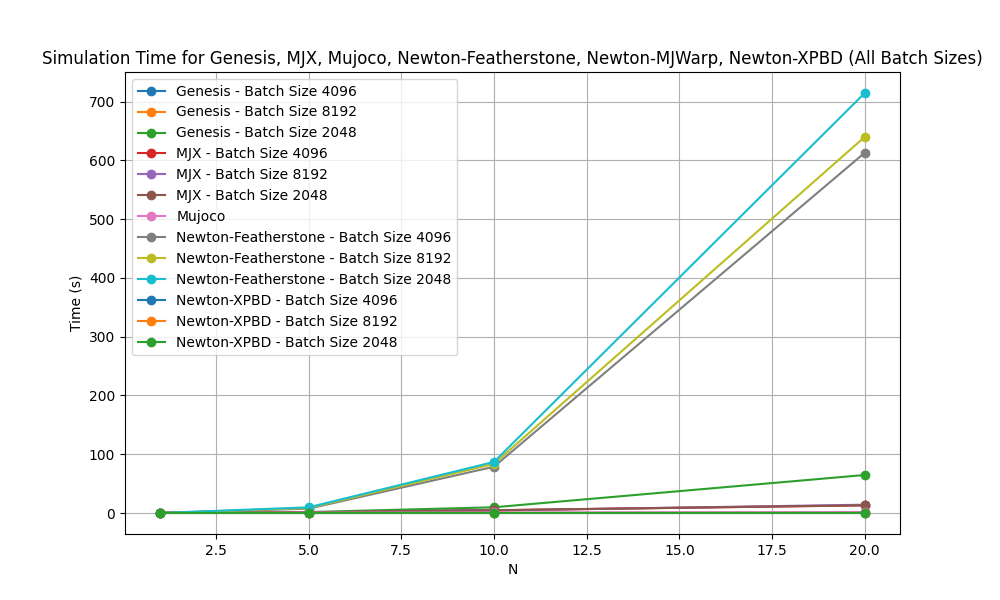
\includegraphics[width=\textwidth]{home/figures/clutter_speed_all.png}
    \caption{Clutter Test: Simulation speed comparison across physics engines.}
    \label{fig:clutter_speed_comparison}
\end{figure}


\subsubsection{Comments:} We see this time that MJWarp failed this test and Genesis failed for N = 20. Regarding MJWarp, it is still under active development and has proven to be unstable even in Newton's official examples.
Genesis doesn't use a sparse matrix approach, which is likely why it struggled with the increased number of DoFs that come with so many environments objects. 6 * 20 * 2048 = 245760, which is a large number of DoFs to simulate via the Jacobian method that Genesis uses. \\
Featherstone performed the worst out of the solvers that didn't fail. \\
Taking a closer look at the other results, we see that MJX, Mujoco and XPBD for Newton performed very well. with MuJoCo outperforming MJX significantly at all batch sizes
\begin{figure}[H]
    \centering
    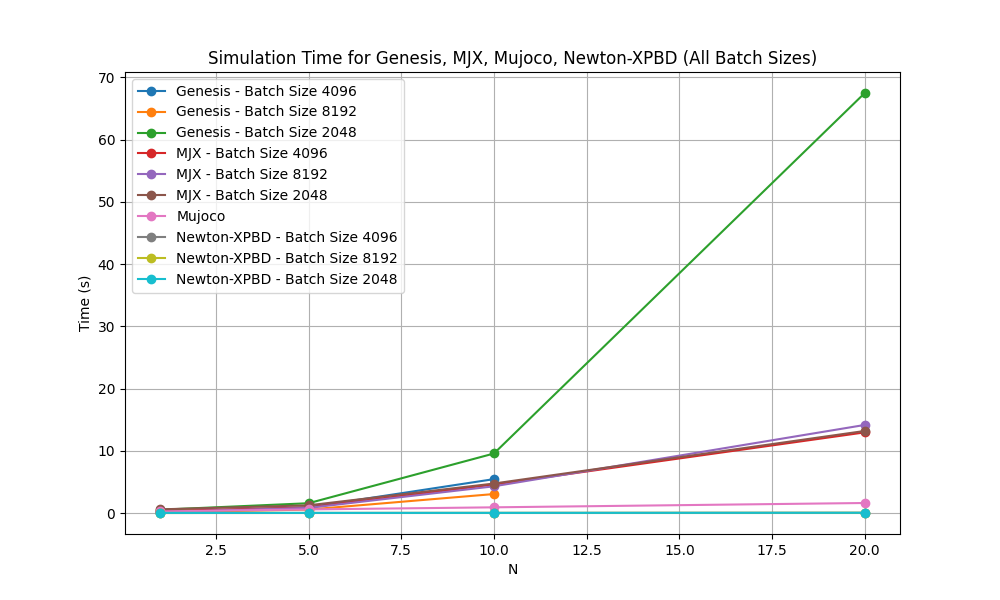
\includegraphics[width=\textwidth]{home/figures/clutter_speed_no-featherstone.png}
    \caption{Clutter Test: Simulation speed comparison across XPBD, MJX, Genesis and MuJoCo.}
    \label{fig:clutter_speed_comparison}
\end{figure}
\noindent XPBD performed the best out of all the solvers for this metric, zooming in further we see that increasing batch size leads to better performance however these returns diminish as N increases.
\begin{figure}[H]
    \centering
    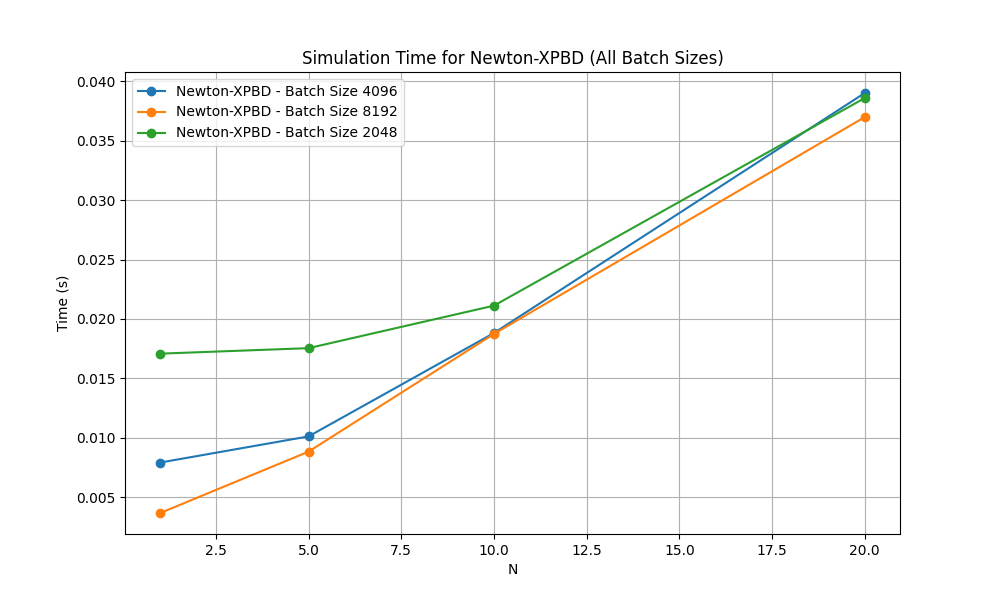
\includegraphics[width=\textwidth]{home/figures/clutter_speed_XPBD.png}
    \caption{Clutter Test: Simulation speed comparison across different batch sizes for XPBD.}
    \label{fig:clutter_speed_comparison}
\end{figure}

\subsection{Increasing Contacts Test}
\begin{figure}[H]
    \centering
    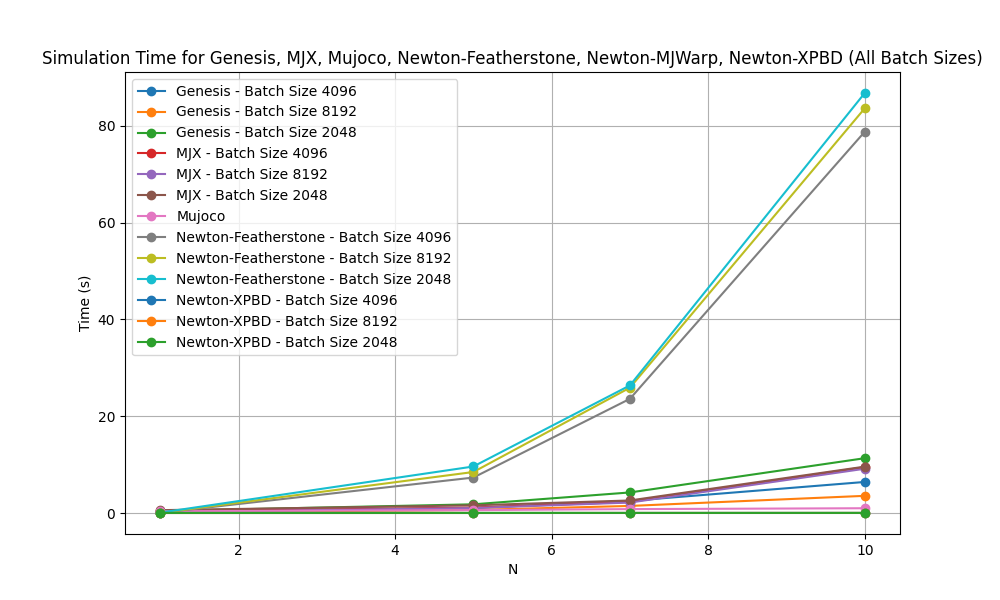
\includegraphics[width=\textwidth]{home/figures/contacts_speed.png}
    \caption{Contacts Test: Simulation speed comparison across physics engines.}
    \label{fig:contacts_speed_comparison}
\end{figure}

\subsubsection{Comments:}
MJWarp failed again, Genesis performed well but it is worth noting that the maximum N tested was 10. Featherstone did the worst out of the solvers that didnt fail, MJX and genesis were again very comparable and MuJoCo only came second to XPBD.

\subsection{Articulation Test}
\begin{figure}[H]
    \centering
    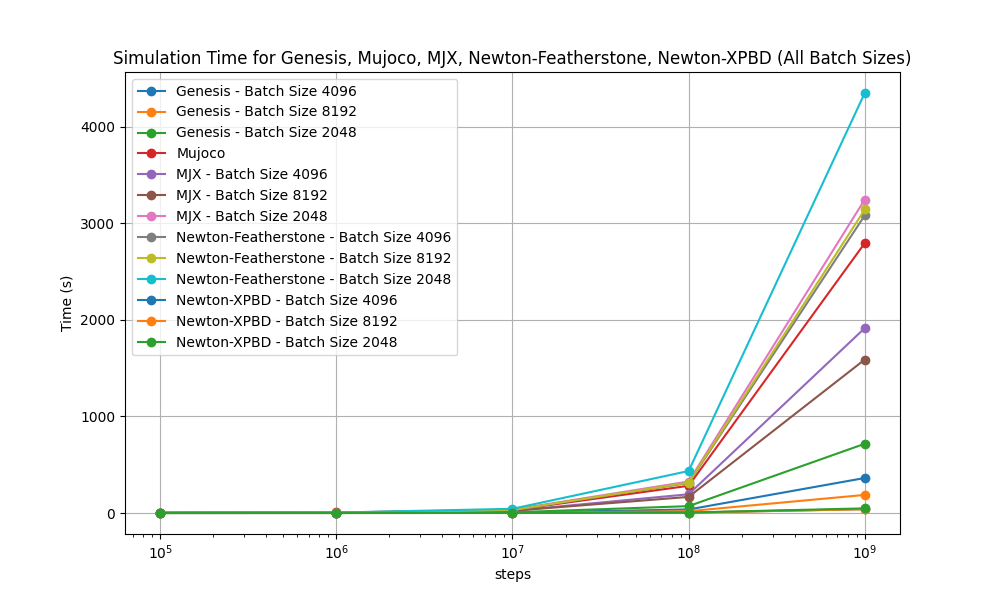
\includegraphics[width=\textwidth]{home/figures/articulation_speed.png}
    \caption{Articulation Test: Simulation speed comparison across physics engines.}
    \label{fig:articulation_speed_comparison}
\end{figure}

\subsubsection{Comments:}
MJWarp failed again, Featherstone did the worst out of the remaining solvers. MuJoCo performed very poorly at high step sizes which shows that it is not suited to high throughput simulations. MJX outperfomed MuJoCo for batch sizes 4096 and 8192. Genesis performed incredibly well but still came second to XPBD.
\begin{figure}[H]
    \centering
    \includegraphics[width=\textwidth]{home/figures/articulation_Newton-Genesis_speed.png}
    \caption{Articulation Test: Close-up simulation speed comparison for XPBD and Genesis.}
    \label{fig:articulation_speed_comparison}
\end{figure}
Here we see that XPBD was by far faster than Genesis, but to reiterate it seems to be a far less physically accurate method so Genesis seems to be the most suitable for high throughput simulations where physical accuracy is critical.

\subsection{Walker Test}
\begin{figure}[H]
    \centering
    %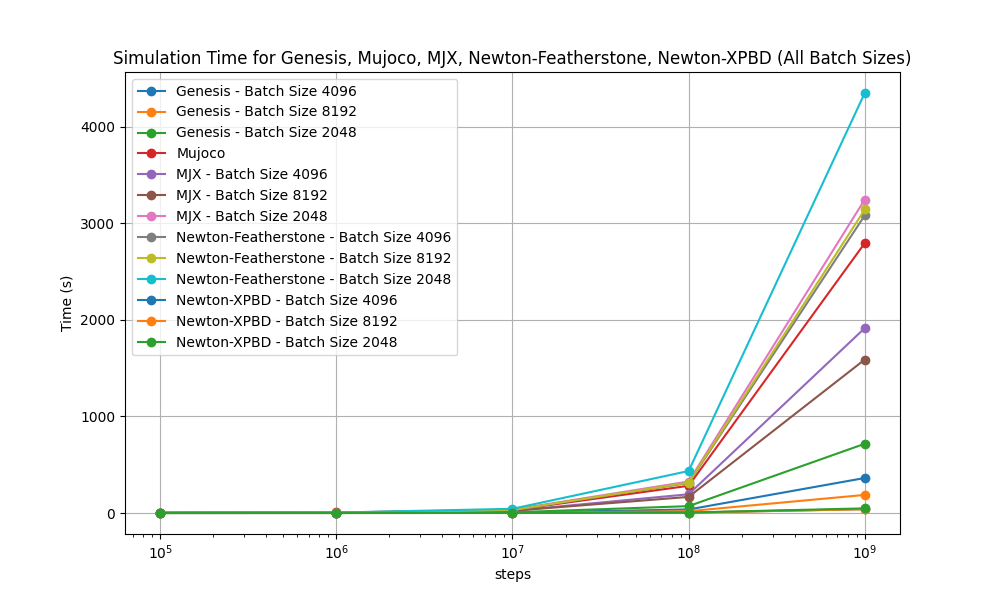
\includegraphics[width=\textwidth]{home/figures/articulation_speed.png}
    %\caption{Articulation Test: Simulation speed comparison across physics engines.}
    %\label{fig:articulation_speed_comparison}
\end{figure}

\subsubsection{Comments:}

\subsection{Loading Times Test}
\begin{figure}[H]
    \centering
    %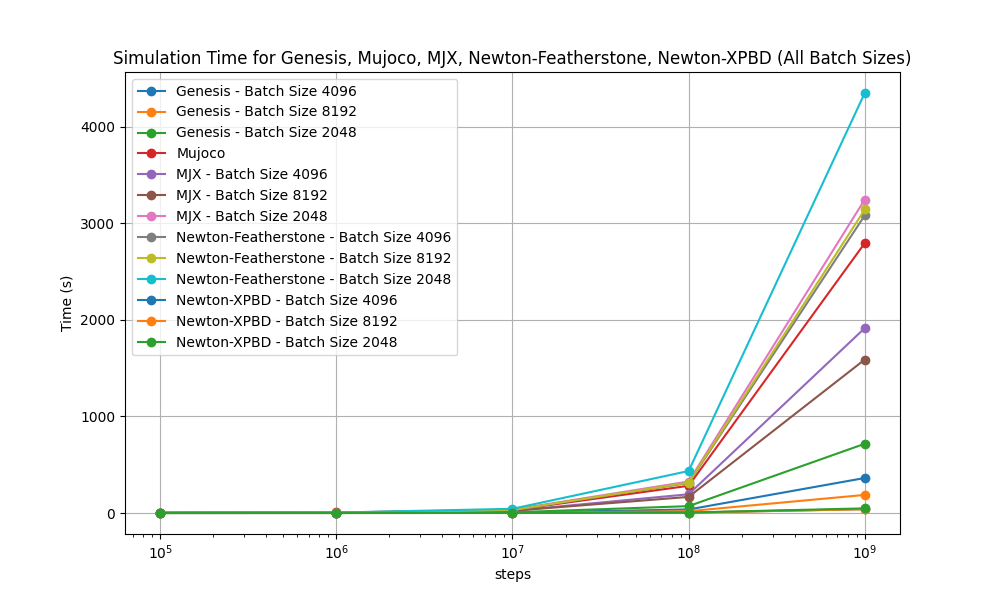
\includegraphics[width=\textwidth]{home/figures/articulation_speed.png}
    %\caption{Articulation Test: Simulation speed comparison across physics engines.}
    %\label{fig:articulation_speed_comparison}
\end{figure}

\subsubsection{Comments:}
\section{Summary}



\bibliographystyle{unsrt}
\bibliography{references}

\end{document}